\begin{align}
7x+3\ &<\ 5x+9 \\
2x - 6\  &< \  0 \\
x &< 3 \\
\therefore\  x\  &\epsilon\  \{3, -\infty \}
\end{align}

\begin{figure}[!ht]
\centering
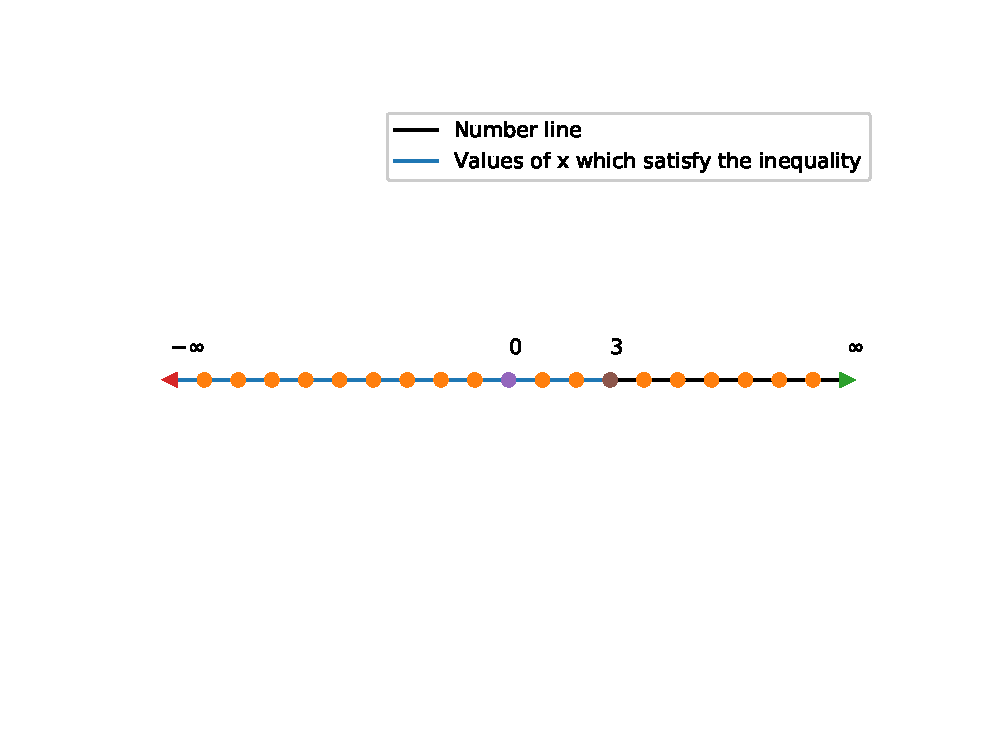
\includegraphics[width=\columnwidth]{./figs/line_ex/lin_ineq/number_line.eps}
\caption{Values of $x$ satisfying the inequality in the number line generated using python}
\label{fig:numberline_lin_ineq}
\end{figure} 

The  following Python code generates Fig. \ref{fig:numberline_lin_ineq}
\begin{lstlisting}
codes/line_ex/lin_ineq/dist_btw_pts.py
\end{lstlisting}



